\subsection{Problem 1}
To get a better controller we want to use an observer to estimate some of the states, rather than using the derivative of the output. To make the observer we need a model of the system with all the states, both measured and those we want to estimate. This model can be written as

\begin{subequations}
	\begin{align*}
		\mbf{\dot x} &= \mbf{A}\mbf{x} + \mbf{B}\mbf{u}\\
		\mbf{y} &= \mbf{C}\mbf{x}
	\end{align*}
\end{subequations}

where the vectors $\mbf{x}$, $\mbf{u}$ and $\mbf{y}$, and the matrices $\mbf{A}$, $\mbf{B}$ and $\mbf{C}$ are given by

\begin{subequations}
	\begin{align}
		\mbf{x} &= \begin{bmatrix}
			\tilde p\\
			\dot{\tilde p}\\
			\tilde e\\
			\dot{\tilde e}\\
			\tilde \lambda\\
			\dot{\tilde \lambda}
			\end{bmatrix}, 
		\mbf{u} = \begin{bmatrix}
			\tilde V_s\\
			\tilde V_d
			\end{bmatrix} \text{and} \ 
		\mbf{y} = \begin{bmatrix}
			\tilde p\\
			\tilde e\\
			\tilde \lambda
			\end{bmatrix}\\
		\mbf{A} &= \begin{bmatrix}
			0 & 1 & 0 & 0 & 0 & 0\\
			0 & 0 & 0 & 0 & 0 & 0\\ 
			0 & 0 & 0 & 1 & 0 & 0\\
			0 & 0 & 0 & 0 & 0 & 0\\
			0 & 0 & 0 & 0 & 0 & 1\\
			K_3 & 0 & 0 & 0 & 0 & 0
			\end{bmatrix}\\
		\mbf{B} &= \begin{bmatrix}
			0 & 0\\
			0 & K_1 &\\
			0 & 0\\
			K_2 & 0\\
			0 & 0\\
			0 & 0	
			\end{bmatrix}\\
		\mbf{C} &= \begin{bmatrix}
			1 & 0 & 0 & 0 & 0 & 0\\
			0 & 0 & 1 & 0 & 0 & 0\\
			0 & 0 & 0 & 0 & 1 & 0
			\end{bmatrix}
	\end{align}
\end{subequations}

\subsection{Problem 2}
Using the MATLAB functions \texttt{obsv(sys)} and \texttt{rank(matrix)} we found that the observability matrix $\mathcal{O}$ have a $\text{rank} = 6$, which is the same as the systems dimension. This means that the system is observable.

We then used the new model to make a linear observer on the form $\mbf{\dot{\hat x}} = \mbf{A}\mbf{\hat x} + \mbf{B}\mbf{u} + \mbf{L} (\mbf{y}-\mbf{C}\mbf{\hat x})$. The observer gain matrix $L$ was found by using the function \texttt{place(A', C', poles).'}. For the controller with integral effect the poles we chose were placed in a fan with a opening of $\frac{\pi}{2}$ radians, and a radius of $20 \cdot r_0$ where $r_0$ is the absolute value of the largest pole of the closed loop system $\mbf{\dot x} = (\mbf{A} - \mbf{B} \mbf{K}) \mbf{x}$. The way we ended up with these poles were by following the recommendations from the lectures of placing them in a fan with a radius sufficiently larger than the absolute value of the largest pole of the cosed loop system, and then trying different radii until we found one that gave a satisfying response. For the controller without integral effect we followed the same procedure, and ended up with the same $\mbf{L}$ matrix.

As the observer does not simply differentiate the output, but also uses it's knowledge of the input it is able to filter out some of the noise. A fast observer will give an accurate estimate, whereas a slow observer will filter out more noise. This means that these benefits needs to be balanced when choosing the poles of the observer. As we can see from \cref{fig:pest}, \cref{fig:pdest}, \cref{fig:eest} and \cref{fig:edest} the observer follows the real values closely, while filters out most of the noise.

\begin{figure}[H]
	\centering
	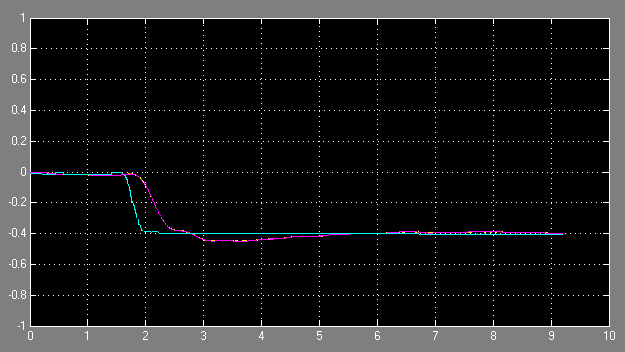
\includegraphics[width=0.95\textwidth]{images/est_med_int/p_est.png}
	\caption{Pitch. Yellow = measurement, red = estimate, blue = reference}
	\label{fig:pest}
\end{figure}
\begin{figure}[H]
	\centering
	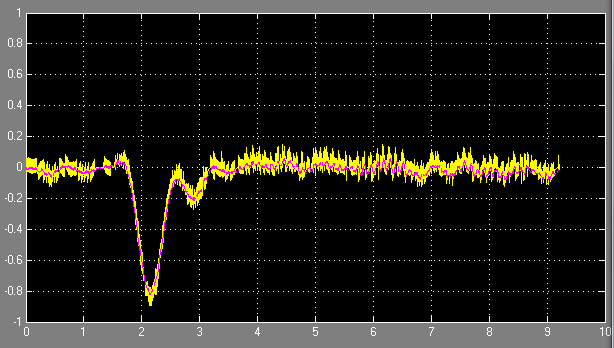
\includegraphics[width=0.95\textwidth]{images/est_med_int/pd_est.png}
	\caption{Pitch rate. Yellow = measurement, red = estimate}
	\label{fig:pdest}
\end{figure}
\begin{figure}[H]
	\centering
	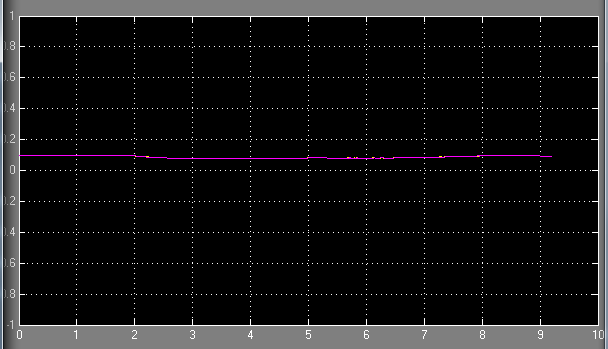
\includegraphics[width=0.95\textwidth]{images/est_med_int/e_est.png}
	\caption{Elevation. Yellow = measurement, red = estimate}
	\label{fig:eest}
\end{figure}
\begin{figure}[H]
	\centering
	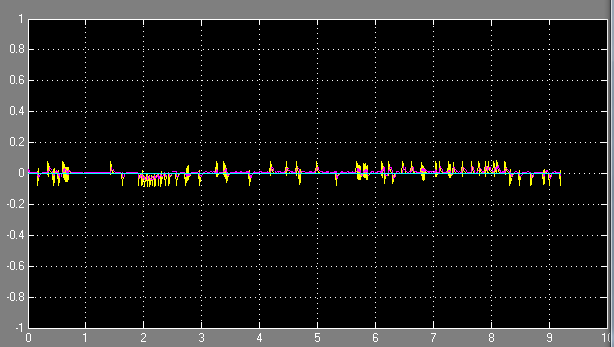
\includegraphics[width=0.95\textwidth]{images/est_med_int/ed_est.png}
	\caption{Elevation rate. Yellow = measurement, red = estimate, blue = reference}
	\label{fig:edest}
\end{figure}


\subsection{Problem 3}
If we only measure $\tilde p$ and $\tilde e$ we we get the following $\mbf{C}$ matrix:

\begin{equation}
	\mbf{C} = \begin{bmatrix}
		0 & 0 & 1 & 0 & 0 & 0\\
		0 & 0 & 0 & 0 & 1 & 0
	\end{bmatrix}
\end{equation}

If we calculate the observer matrix $\mathcal{O}$ we get that the rank is 6, which means that the system is observable. However, we found that the observer is too bad to be used to control the helicopter. The reason for the bad estimates is that we control the pitch and pitch rate which are not measured. This means that we try to estimate states that are the second and third derivative of one of the states that we measure, namely travel. This means that even though it is theoretically possible to control the system, it is very hard to make a good controller that works well on the real system. Another reason why the estimates are poor are because the estimator is based on a linear model, while the real system is non-linear. Even though we weren't able to control the system, we were at least able to get the estimator stable, and when we hold the helicopter down, all the estimates go towards the right values.